\documentclass[11pt,twocolumn]{article}
\usepackage{lmodern,setspace,amsmath,amssymb,amsfonts,amsthm,graphicx,multicol}
\usepackage[a4paper, top=0.9in, bottom=1.15in]{geometry}
\usepackage[polish]{babel}
\usepackage[utf8]{inputenc}
\title{Algorytmy i struktury danych - Algorytmy z powracaniem}
\author{Dariusz Max Adamski}
\date{}

\begin{document}

\maketitle


\section*{Wstęp}

W tym sprawozdaniu mierzony będzie czas poszukiwania
cyklu Eulera i Hamiltona w grafie nieskierowanym,
w zależności od ilości wierzchołków oraz nasycenia krawędziami.


\section*{Metodologia}

Pomiary czasu znajdywania cyklu Eulera ,,EC'' i Hamiltona ,,HC'' wykonywane były na grafach
o ilości wierzchołków $|V|$ od $200$ do $1\ 000$ wierzchołków, z krokiem $200$ (5 grup pomiarów).
W każdej grupie wykonywane były pomiary na grafach o nasyceniu krawędziami
$\varphi \in \{0.1, 0.2, 0.3, 0.4, 0.6, 0.8, 0.95\}$.
Czas poszukiwania HC był mierzony 25 razy dla każdej pary $\langle |V|, \varphi \rangle$.
Każdy pomiar wykonywany był na nowym losowo wygenerowanym grafie.

Przed mierzeniem czasu wczytywany jest, z pliku tekstowego,
losowo wygenerowany, nieskierowany, spójny graf eulerowski,
o ilości wierzchołków $|V|$  i nasyceniu krawędziami $\varphi$,
do macierzy sąsiedztwa ,,AM''.

Optymalizacje kompilatora zostały wyłączone flagą ,,-O0''. 
Czas wykonywania był mierzony w nanosekundach.


\section{Cykl Eulera}

\begin{figure}[h]
	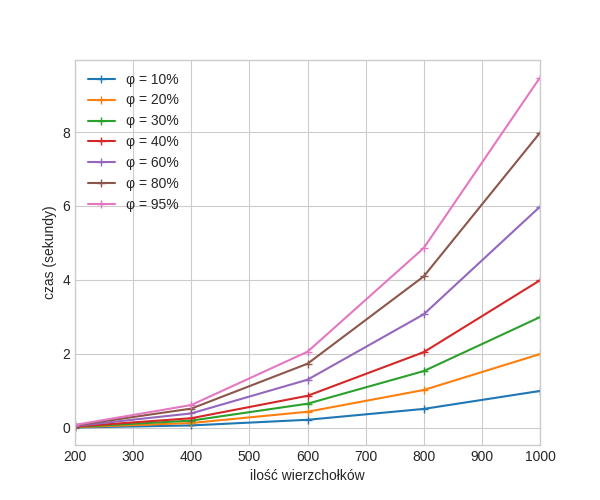
\includegraphics[width=\linewidth]{euler.png}
	\caption{Czas znajdywania cyklu Eulera, w zależności od $|V|$ \label{euler}}
\end{figure}

Dla nieskierowanego, eulerowskiego grafu, czas znajdywania EC
ma złożoność $O(|E|) = O(|V|^2)$, co widać na rysunku \ref{euler}.

Do reprezentacji grafu użyta została macierz sąsiedztwa.
Głównym powodem była prostota generowania grafu.
Ponadto, ponieważ musimy przechowywać grafy o dużym $\varphi$,
korzystająć z AM oszczędzamy trochę pamięci.
Alternatywnie mogła zostać wybrana lista incydencji, co
minimalnie uprościłoby kod,
oraz nieznacznie zmniejszyłoby czas wykonywania.
Inne reprezentacje grafu są niepraktyczne ze względu na złożoność pamięciową,
lub złożoność operacji sprawdzania istnienia krawędzi.

\section{Cykl Hamiltona}

\begin{figure}[h!]
	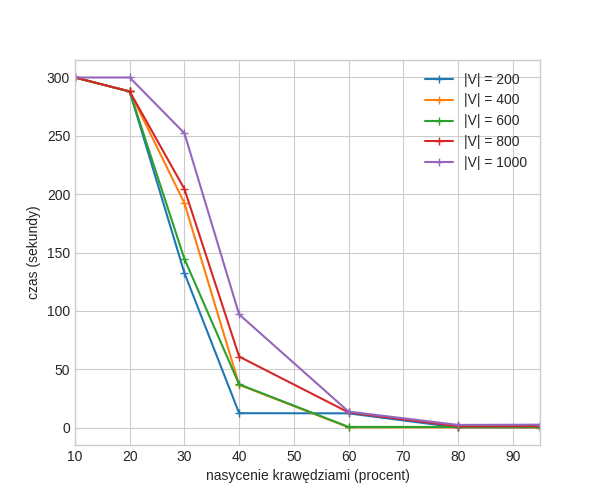
\includegraphics[width=\linewidth]{hamil_by_v.png}
	\caption{Czas znajdywania cyklu Hamiltona, w zależności od $\varphi$ \label{hamil_by_v}}
\end{figure}

\begin{figure}[h!]
	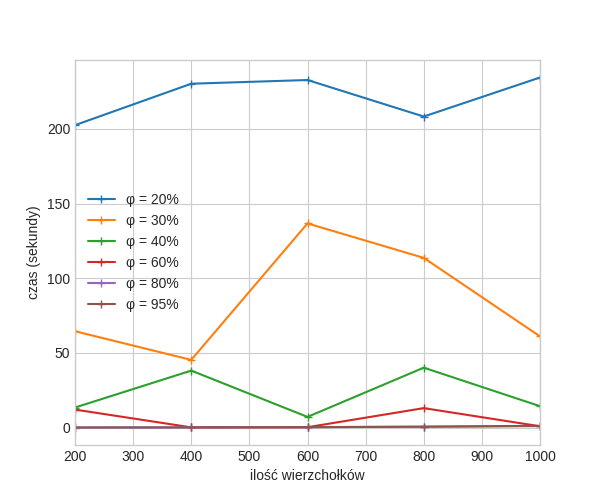
\includegraphics[width=\linewidth]{hamil.png}
	\caption{Czas znajdywania cyklu Hamiltona, w zależności od $|V|$ \label{hamil}}
\end{figure}

Czas znajdywania HC ma złożoność $O(|V|!)$.
Wyniki są przedstawione w zależności od $\varphi$ na rysunku 2,
oraz od $|V|$ na rysunku 3.
Grafy o małym nasyceniu krawędziami stanowią najgorsze przypadki.
Wtedy czas znajdywania HC przekracza ustalony limit $300$ sekund.
Ze wzrostem ilości krawędzi, spada czas wymagany do znalezienia cyklu.
Przy $\varphi = 0.95$, znalezienie HC zajmuje średnio jedną sekundę.
Ewentualne odchylenia są spowodowane losowością wygenerowanych grafów.

\end{document}

